No planeta AnThais, os AnThaisianos habitualmente são seres de Luz sem forma.

Movem-se deslizando e gerando um campo energético de brilho e cores desconhecidas na Terra.

Para poderem ter uma ideia, só um bocadinho aproximada, do que é o ambiente de AnThais, visto que os terráqueos precisam visualizar para compreender, imaginem, no chão e num dia de vento, uma poça de água limpa mesclando-se com óleo derramado e a sua superfície está exposta ao Sol, que se reflete nela.

As cores desta mistura ficam brandas, visíveis, mas sem estarem individualizadas. E o vento faz aparecer imagens desfocadas num contínuo movimento de plasma, que gera mais cores e mais desenhos.

Esta analogia é apenas uma pincelada para a imaginação, porque é indescritível colocar em palavras o que não é deste mundo.

Assim, os AnThaisianos são a tal Unidade, funcionando como um Todo sem jamais perderem a Individualidade. Mas a individualidade para eles não existe, porque são um por todos e todos por um.

Comunicam-se instantaneamente e todos sabem o que cada um pensa e sente.

Mas como são a Unidade, não precisam trocar pensamentos.

Vivem em Harmonia porque são Amor. E porque são Amor emitem Luz. A Luz que os conduz novamente até ao Amor.

São viajantes cósmicos por natureza e fazem-no sempre com a mesma Alegria interior, sem distinguir os mundos que visitam.

E no espaço sideral, que só termina no infinito, há zilhões de mundos a visitar.
\bigbreak
O sol desloca-se mais um palmo no céu, está calor.
\bigbreak
\textbf{Eu sou Eu} e os insetos estão deitados no relvado, pernas esticadas e braços abertos. Riram tanto, mas tanto, que ficaram em estado de completude. Plenos de Alegria.
\bigbreak

\begin{figure}[h]
    \centering
    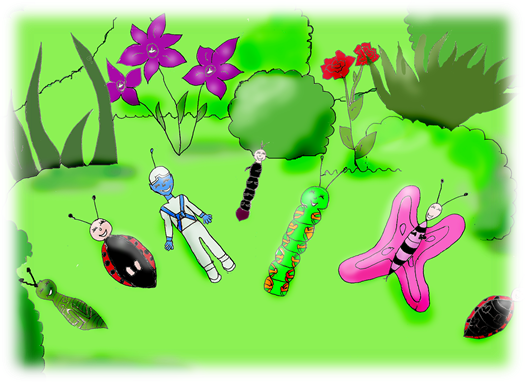
\includegraphics[width=0.85\textwidth]{deitados}
\end{figure}

O riso é uma terapia. O mundo inteiro devia rir.
\bigbreak
— Porque escolheste o nosso jardim? – pergunta uma borboleta.
\bigbreak
— Muito simples! – diz \textbf{Eu sou Eu} - Eu só posso entrar em contato com alguém que sintonize de alguma forma com o meu Mundo. E o mundo dos insetos preenche esse requisito. No planeta Terra existem mais formas de vida com a mesma sintonia de AnThais, mas... nem todas são assim.

— É verdade, é verdade! – surgem várias vozes em conjunto. E uma formiguita continua com a linha de pensamento do grupo.

— Os humanos não têm essa frequência. Tudo o que para eles é desconhecido e que sai da sua rotina, mete-lhes medo, deixando-os desconfiados. E aos seres que não são gente como eles, tratam como inferiores. Eles acham-se os donos da Terra. Recolhem e acartam, tudo o que podem para dentro das suas casas, quer precisem, quer não precisem! E até a Mãe Gaia não percebe porque eles agem assim. Afinal, ela está continuamente a produzir alimentos, por cada poro seu, seja na terra, seja no mar, para todas as criaturas que nela habitam. A Abundância é enorme. Chega para todos e sobra sempre. Mas eles acham que não.
\bigbreak
Uma joaninha pega na conversa:
\bigbreak
— E como nos perseguem? Adoram apanhar insetos e meter-nos em frascos e caixas! E depois deixam-nos ali esquecidos sem nos abrirem as prisões. Mas acabamos por nos divertir quando vemos as caras que fazem, com o nariz colado ao frasco, olhando para nós.

— Isso é porque são vocês, Joaninhas. A nós, formigas, simplesmente exterminam-nos deste mundo. Mas não faz mal, aparecemos noutro lado. A nossa Consciência jamais pode ser aniquilada.
\bigbreak
\textbf{Eu sou Eu} sente-se em casa porque aquele oceano de pequenos insetos tem uma Enorme Consciência de Si e do que os rodeia. Então diz:
\bigbreak
— Só uma minoria dos humanos consegue ver o que é óbvio: o que fazem à mais pequena das criaturas é feito igualmente ao seu Criador! Grande parte desta humanidade ainda dorme com os olhos abertos. Todos os Reinos deste mundo, o mineral, o vegetal e o animal, que aqui habitam e são Unidade percebem isso, com exceção dos homens que poluem, destroem, devastam o que a Mãe Gaia lhes oferta com Amor! E ainda por cima se julgam superiores e inteligentes! Não acham esta a maior piada neste mundo?
\bigbreak
E mais uma vez desatam todos a rir às gargalhadas.

Sim, só pode mesmo ser uma anedota.
\bigbreak
Não é à toa que as crianças pequenas não percebem o mundo dos grandes. Porque elas têm a capacidade de ver com o coração, um Mundo que é invisível aos olhos dos adultos.
\bigbreak
Veem que tudo nesta vida está em conexão, como o tal plasma colorido que se move sem parar.

Veem que quando uma borboleta voa, o movimento gerado pelas suas delicadas asas gera um turbilhão no outro lado do planeta.
\bigbreak
Que há uma explosão de Amor, quando uma pequena e frágil flor se oferta ao Sol, abrindo as suas pétalas para o abraçar.
\bigbreak
Que o que é feio e desconcertante no mundo, desaparece quando se fecham os olhos da cara e se abrem os do Coração.
\bigbreak
As crianças vivem no Hoje, sem pensar no que já passou e sem se preocupar com o amanhã, porque simplesmente eles não existem.
\bigbreak
O riso ainda estava no ar quando \textbf{Eu sou Eu} recomeça a falar:
\bigbreak
— Quando decidi fazer esta viagem quis experimentar uma ET. São naves de pequeno tamanho, logo eu teria de ser pequenote para viajar nela. E ninguém melhor que vocês para me receberem!
\bigbreak
Uma onda de gratidão emana dos insetos.

\textbf{Eu sou Eu} dá um suspiro. Estão em sintonia.

E por falar em sintonia, uma formiga pergunta:
\bigbreak
— Por que é que só tens uma antena na tua cabeça? Nós temos sempre duas! Servem-nos de radar para nos localizarmos e são muito importantes para nos cumprimentarmos umas às outras.

O AnThaisiano delicia-se com a simplicidade dos insetos. Então explica:
\bigbreak
— A antena que veem é a minha ligação com o meu mundo. Através dela eu comunico com AnThais e recebo informações quando necessário. Mantém-nos em Unidade quando viajamos para mundos desligados, dualitários, como a Terra. Sempre que preciso de alguma coisa, basta-me sintonizá-la e é imediato o resultado.

— Como eu gostaria de ter uma antena assim! – diz a mesma formiga.

— Eu preciso de duas assim! Cada salto que dou e o vento me leva... fico sem saber onde estou. – fala um gafanhoto que é meio deslocalizado.
\bigbreak
\textbf{Eu sou Eu} sente um prazer imenso, aqueles insetos não são deste mundo!

Um deles pergunta:

— E a tua forma no planeta AnThais é sempre sem forma?
\bigbreak
\begin{figure}[h]
    \centering
    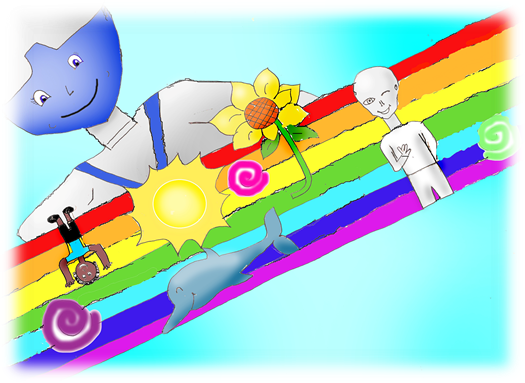
\includegraphics[width=0.85\textwidth]{arco_iris}
\end{figure}


 — Não! No meu planeta, como também já falei, todos somos luz, mas podemos assumir qualquer aparência. Quando isso acontece, escolhemos... bem… como hei-de explicar... escolhemos um disfarce, uma máscara. A tonalidade dela é sempre azulada, porque está em relação com o nosso sol – Sírius! Mas a forma pode ser qualquer uma. Posso ser mesmo uma lagarta ou uma borboleta. Posso ser uma nuvem. Ou uma menina como a Joana. Ou outras formas que são desconhecidas aqui na Terra. Quando nos mascaramos com uma forma é simplesmente para nos divertirmos, para brincarmos. É uma Alegria enorme fazê-lo. E contagiamos todos.
 \bigbreak
\textbf{Eu sou Eu} para de falar e olha com ternura o jardim. Neste momento, a Joana abre novamente a porta de casa e sai a correr, trazendo na mão um cata-vento a girar. Quando se encontra no meio do jardim, procura uma brisa para o seu brinquedo.

O vento está atento e corre para ela.

O cata-vento volta a rodar sem parar e a menina sorri.

\textbf{Eu sou Eu} retoma a conversa:
\bigbreak
— Portanto, aqui na Terra, se os humanos conseguissem atingir mentalmente o que significa estar mascarado, ter forma, que não é mais que uma brincadeira, este mundo seria igualmente perfeito! Mas confundem as suas máscaras com o que são em Essência, identificam-se com as personagens que interpretam e assim levam tudo muito a sério. Se apreendessem que o mundo em que vivem é um palco onde se desenrola uma peça de teatro gigante, onde todos participam, passariam a brincar e a viver em alegria, como fazem as crianças. Compreenderiam que no palco do teatro da Vida há objetos e obstáculos em que podem tropeçar e se magoar e que basta estar atento e presente, contornando-os, para isso não acontecer. Passariam a andar mais sorridentes, em vez de estarem sempre com um ar sisudo de preocupação.

O sol começa a sua descida no céu.

O vento mantém-se suave.

As árvores zeladoras.

E a menina, de pés descalços, entrega-se com prazer ao momento presente.
